\documentclass[border=8pt]{standalone}
\usepackage[T1]{fontenc}\usepackage{helvet}\renewcommand{\familydefault}{\sfdefault}
\usepackage{tikz}\usetikzlibrary{arrows.meta, positioning, calc, backgrounds}
\definecolor{ink}{HTML}{1a1916}
\definecolor{inktwo}{HTML}{3a3a35}
\definecolor{inkthree}{HTML}{6a6862}
\definecolor{rule}{HTML}{b8b09a}
\definecolor{amber}{HTML}{a8730a}
\definecolor{red}{HTML}{c8261a}
\definecolor{paper}{HTML}{f0eee5}
\definecolor{slab}{HTML}{d8d4c6}
\tikzset{
  >={Stealth[length=2.2mm]},
  wire/.style={line width=0.8pt, ink},
  modwire/.style={line width=0.6pt, dashed, ink},
  tastewire/.style={line width=0.6pt, dashed, amber},
  gatewire/.style={line width=0.6pt, dotted, ink},
  block/.style={rectangle, draw=ink, line width=0.9pt, fill=slab, minimum width=3.0cm, minimum height=1.9cm, inner sep=0pt},
  perf/.style={rectangle, draw=ink, line width=0.7pt, minimum width=3.0cm, minimum height=0.7cm, inner sep=2pt, font=\footnotesize, text=ink},
  title/.style={font=\scriptsize\bfseries, text=ink, anchor=north, inner sep=2pt},
  jack/.style={circle, draw=ink, fill=paper, line width=0.5pt, minimum size=3.2pt, inner sep=0pt},
  plabel/.style={font=\tiny, text=inktwo, anchor=west, inner sep=1pt},
  olabel/.style={font=\tiny, text=inktwo, anchor=east, inner sep=1pt},
  settings/.style={font=\scriptsize, text=ink, align=left, anchor=north west, inner sep=1pt, text width=2.9cm},
}
\begin{document}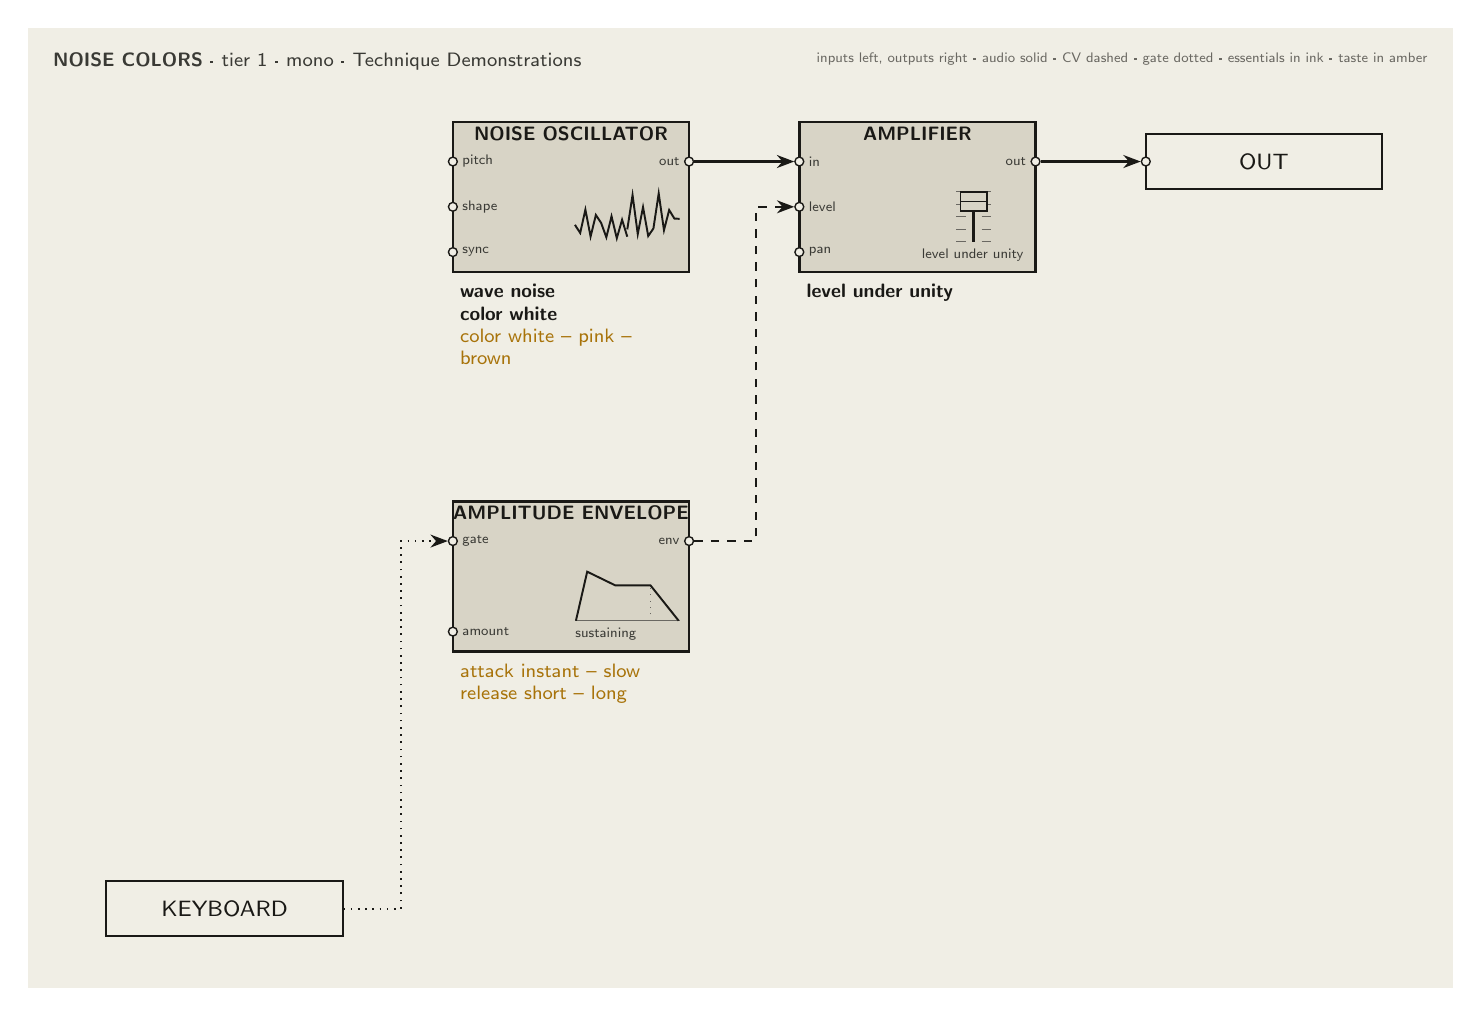
\begin{tikzpicture}
\begin{scope}[on background layer]\fill[paper] (-2.5,-10.040000000000001) rectangle (15.600000000000001,2.15);\end{scope}
\node[block, minimum height=1.9cm] (noise) at (4.4,0.0) {};
\node[title] at (noise.north) {NOISE OSCILLATOR};
\node[jack] (noise-pitch) at (2.9000000000000004,0.44999999999999996) {};
\node[plabel] at (2.9800000000000004,0.44999999999999996) {pitch};
\node[jack] (noise-shape) at (2.9000000000000004,-0.125) {};
\node[plabel] at (2.9800000000000004,-0.125) {shape};
\node[jack] (noise-sync) at (2.9000000000000004,-0.7) {};
\node[plabel] at (2.9800000000000004,-0.7) {sync};
\node[jack] (noise-out) at (5.9,0.44999999999999996) {};
\node[olabel] at (5.82,0.44999999999999996) {out};
\begin{scope}
\draw[ink, line width=0.7pt] (4.450,-0.354) -- (4.517,-0.457) -- (4.583,-0.161) -- (4.649,-0.503) -- (4.716,-0.229) -- (4.783,-0.330) -- (4.849,-0.512) -- (4.915,-0.246) -- (4.982,-0.524) -- (5.049,-0.289) -- (5.115,-0.505);
\draw[ink, line width=0.7pt] (5.115,-0.412) -- (5.182,0.024) -- (5.248,-0.471) -- (5.315,-0.129) -- (5.381,-0.496) -- (5.447,-0.400) -- (5.514,0.045) -- (5.581,-0.422) -- (5.647,-0.166) -- (5.713,-0.274) -- (5.780,-0.278);
\end{scope}
\node[settings] at (2.95,-1.0699999999999998) {\textbf{wave noise} \\ \textbf{color white} \\ \textcolor{amber}{color white -- pink -- brown}};
\node[block, minimum height=1.9cm] (amp) at (8.8,0.0) {};
\node[title] at (amp.north) {AMPLIFIER};
\node[jack] (amp-in) at (7.300000000000001,0.44999999999999996) {};
\node[plabel] at (7.380000000000001,0.44999999999999996) {in};
\node[jack] (amp-level) at (7.300000000000001,-0.125) {};
\node[plabel] at (7.380000000000001,-0.125) {level};
\node[jack] (amp-pan) at (7.300000000000001,-0.7) {};
\node[plabel] at (7.380000000000001,-0.7) {pan};
\node[jack] (amp-out) at (10.3,0.44999999999999996) {};
\node[olabel] at (10.22,0.44999999999999996) {out};
\begin{scope}
\draw[ink, line width=1.2pt] (9.515,-0.570) -- (9.515,0.070);
\draw[inkthree, line width=0.3pt] (9.295,-0.570) -- (9.415,-0.570) (9.615,-0.570) -- (9.735,-0.570);
\draw[inkthree, line width=0.3pt] (9.295,-0.410) -- (9.415,-0.410) (9.615,-0.410) -- (9.735,-0.410);
\draw[inkthree, line width=0.3pt] (9.295,-0.250) -- (9.415,-0.250) (9.615,-0.250) -- (9.735,-0.250);
\draw[inkthree, line width=0.3pt] (9.295,-0.090) -- (9.415,-0.090) (9.615,-0.090) -- (9.735,-0.090);
\draw[inkthree, line width=0.3pt] (9.295,0.070) -- (9.415,0.070) (9.615,0.070) -- (9.735,0.070);
\fill[slab, draw=ink, line width=0.6pt] (9.345,-0.178) rectangle (9.685,0.062);
\draw[ink, line width=0.5pt] (9.345,-0.058) -- (9.685,-0.058);
\node[font=\tiny, text=inktwo, anchor=north west, inner sep=0pt] at (8.850,-0.650) {level under unity};
\end{scope}
\node[settings] at (7.3500000000000005,-1.0699999999999998) {\textbf{level under unity}};
\node[block, minimum height=1.9cm] (aenv) at (4.4,-4.82) {};
\node[title] at (aenv.north) {AMPLITUDE ENVELOPE};
\node[jack] (aenv-gate) at (2.9000000000000004,-4.37) {};
\node[plabel] at (2.9800000000000004,-4.37) {gate};
\node[jack] (aenv-amount) at (2.9000000000000004,-5.52) {};
\node[plabel] at (2.9800000000000004,-5.52) {amount};
\node[jack] (aenv-out) at (5.9,-4.37) {};
\node[olabel] at (5.82,-4.37) {env};
\begin{scope}
\draw[inkthree, line width=0.3pt] (4.450,-5.381) -- (5.780,-5.381);
\draw[ink, line width=0.7pt] (4.463,-5.381) -- (4.606,-4.759) -- (4.963,-4.933) -- (5.410,-4.933) -- (5.767,-5.381);
\draw[inkthree, line width=0.3pt, dotted] (5.410,-5.381) -- (5.410,-4.933);
\node[font=\tiny, text=inktwo, anchor=north west, inner sep=0pt] at (4.450,-5.470) {sustaining};
\end{scope}
\node[settings] at (2.95,-5.890000000000001) {\textcolor{amber}{attack instant -- slow} \\ \textcolor{amber}{release short -- long}};
\node[perf] (key) at (0.0,-9.040000000000001) {KEYBOARD};
\node[perf, fill=paper] (out) at (13.200000000000001,0.44999999999999996) {OUT}; \node[jack] (out-in) at (11.700000000000001,0.44999999999999996) {};
\draw[wire,->] (noise-out) -- (amp-in);
\draw[wire,->] (amp-out) -- (out-in);
\draw[modwire,->] (aenv-out) -- (6.750000000000001,-4.37) -- (6.750000000000001,-0.125) -- (amp-level);
\draw[gatewire,->] (key.east) -- (2.2400000000000007,-9.040000000000001) -- (2.2400000000000007,-4.37) -- (aenv-gate);
\node[anchor=north west, font=\scriptsize, text=inktwo] at (-2.3,1.95) {\textbf{NOISE COLORS} · tier 1 · mono · Technique Demonstrations};
\node[anchor=north east, font=\tiny, text=inkthree] at (15.400000000000002,1.95) {inputs left, outputs right · audio solid · CV dashed · gate dotted · essentials in ink · taste in amber};
\end{tikzpicture}\end{document}
